\chapter{Resultados e Discussão}

Nesta seção apresentamos os resultados obtidos a partir da análise das coautorias, onde são discutidos os resultados relacionados à produção bibliográfica, impacto e colaboração com as demais áreas, além da interdisciplinaridade da Ciência da Computação, comparando-a com as demais áreas e discutindo como suas relações acontecem sob o ponto de vista das coautorias.

\section{Produção bibliográfica}

O número de publicações científicas únicas feitas em coautoria com pesquisadores da Ciência da Computação é de $282.796$, sendo a 5ª área que mais colabora considerando as publicações de todos os tempos, ficando atrás apenas da Medicina, Agronomia, Educação e Química, como mostra a \autoref{tab:producaoporarea}.

\begin{table}[htpb]
    \centering
    \caption{As 10 áreas que mais produzem publicações científicas em coautoria na ciência brasileira.}
    \label{tab:producaoporarea}
    \begin{tabular}{|r|l|c|}%
        \hline & Área & Número de publicações\\\hline
        \csvreader[late after line=\\\hline]%
        {"tabelas/resultados-producao-bliografica-por-area.csv"}%
        {area=\area,contagem=\contagem}%
        {\thecsvrow & \area & \contagem}%
    \end{tabular}
\end{table}

A \autoref{fig:coautoriaanual} apresenta um gráfico de segmento anual, que vai do ano de surgimento do Currículo Lattes até o último ano completo, indicando crescimento no número de publicações feitas em coautoria. Nele é possível observar que o crescimento do número de coautorias da Ciência da Computação acompanhou as demais áreas do conhecimento.

São exceções as áreas de Educação e Medicina que, durante os períodos de 2003-2009 e 2002-2006, respectivamente, tiveram crescimento acelerado, mas depois se mantiveram estáveis. Ainda, é importante pontuar que a queda acentuada no número de publicações no ano de 2018, presente em todas as áreas, provavelmente está relacionada ao fato de a coleta ter sido feita no início de 2019, quando as publicações do ano de 2018 não haviam sido totalmente concluídas.

\begin{figure}[htpb]
  \centering
  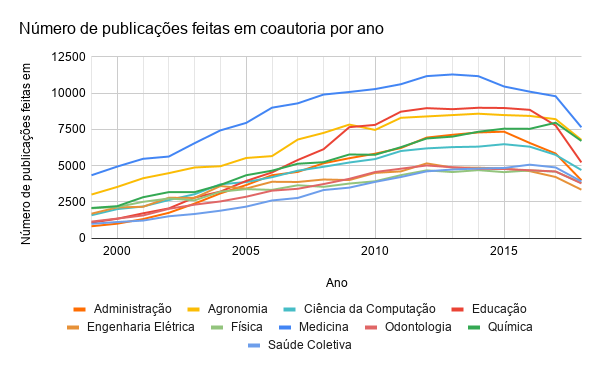
\includegraphics[width=1\textwidth]{figuras/resultados-grafico-coautoria-anual}
  \caption{Gráfico de segmento anual com a produção em coautoria das áreas que mais produzem em coautoria no período de 1999 a 2018.}
  \label{fig:coautoriaanual}
\end{figure}

\section{Impacto e colaboração}

A rede de coautoria entre as áreas do conhecimento apresentada na \autoref{fig:grafocolaboracao} foi construída a partir das redes de coautorias entre os pesquisadores. O diâmetro da rede é igual a $3$, o caminho médio igual a $1,31$ e coeficiente médio de clusterização igual a $0,912$. Essa rede apresenta um comportamento comumente observado em redes sociais, é coesa e se caracteriza pela alta densidade de arestas, indicando que quase todas as áreas do conhecimento estão relacionadas entre si. Este fato observado se comporta como o esperado, dado que na ciência não se trabalha de forma isolada.

\begin{figure}[htpb]
  \centering
  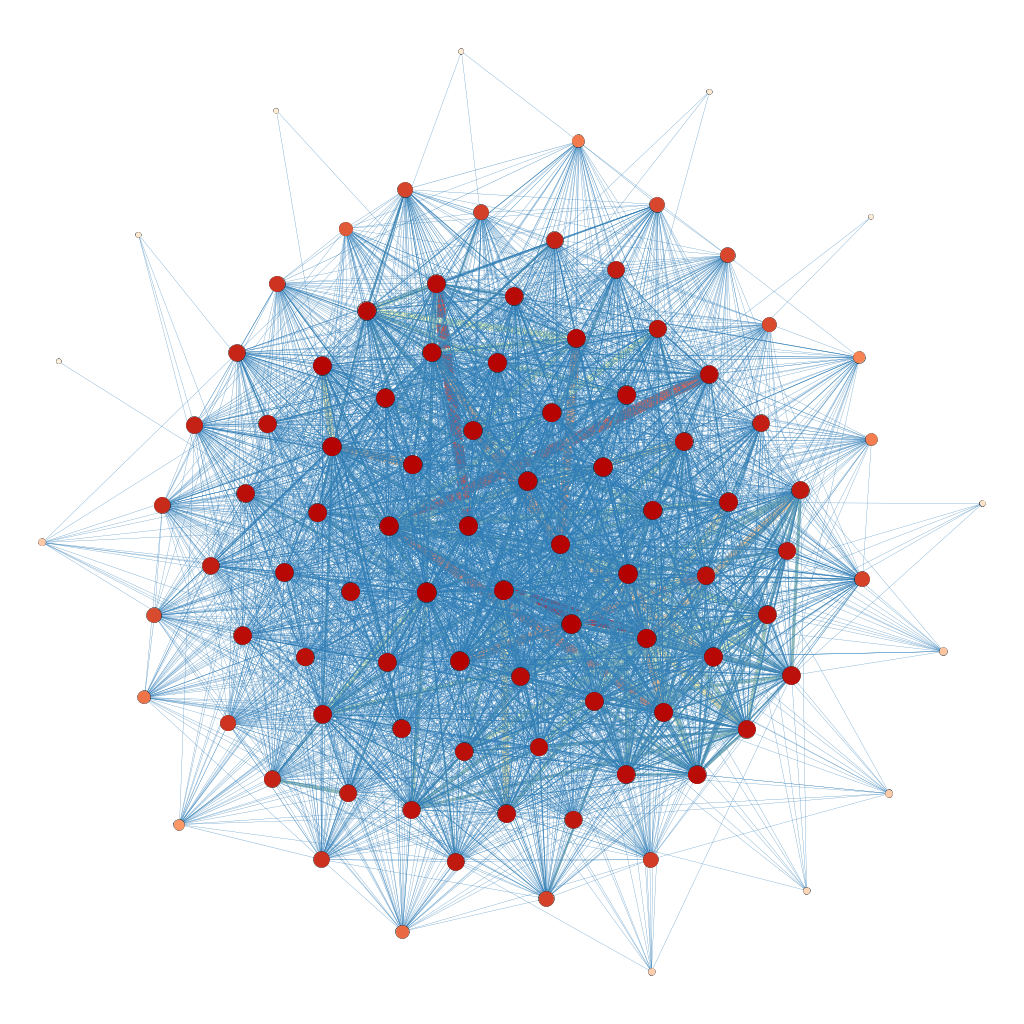
\includegraphics[width=1\textwidth]{figuras/resultados-grafo-colaboracao-entre-areas}
  \caption{Rede de coautoria entre as áreas do conhecimento.}
  \label{fig:grafocolaboracao}
\end{figure}

O mapa de calor da \autoref{fig:mapadecalorcolaboracao}, com as coautorias feitas entre as áreas, mostra que o maior esforço de colaboração da Ciência da Computação está com a Engenharia Elétrica, sendo que as áreas mais impactadas pela Ciência da Computação são a Matemática, Engenharia Elétrica e Ciência da Informação. Ainda segundo este mapa, podemos verificar que a Medicina é a área que mais impacta áreas distintas.

\begin{landscape}
  \begin{figure}[htbp]
    \centering
    \includegraphics[width=\linewidth, height=\textheight, keepaspectratio]%
    {figuras/resultados-mapa-de-calor-colaboracao-entre-areas}
    \caption{Mapa de calor das colaborações exercidas entre as áreas do conhecimento. As linhas podem ser interpretadas como o esforço exercido na colaboração e as colunas como o esforço percebido pelas outras área na colaboração. Colunas com maior atividade são as áreas que mais impactam as outras.}
    \label{fig:mapadecalorcolaboracao}
  \end{figure}
\end{landscape}

Uma visualização que permite observar o impacto exercido por cada área é apresentada na \autoref{fig:grafoimpacto}. Esta é uma interpretação do mapa de calor de colaboração entre as áreas, onde os nós são as áreas do conhecimento e as arestas direcionadas representam o impacto exercido por uma área do conhecimento em outra, isto é, quanto das suas coautorias realizadas determinam a produção das publicações científicas das outras áreas.

\begin{figure}[htpb]
  \centering
  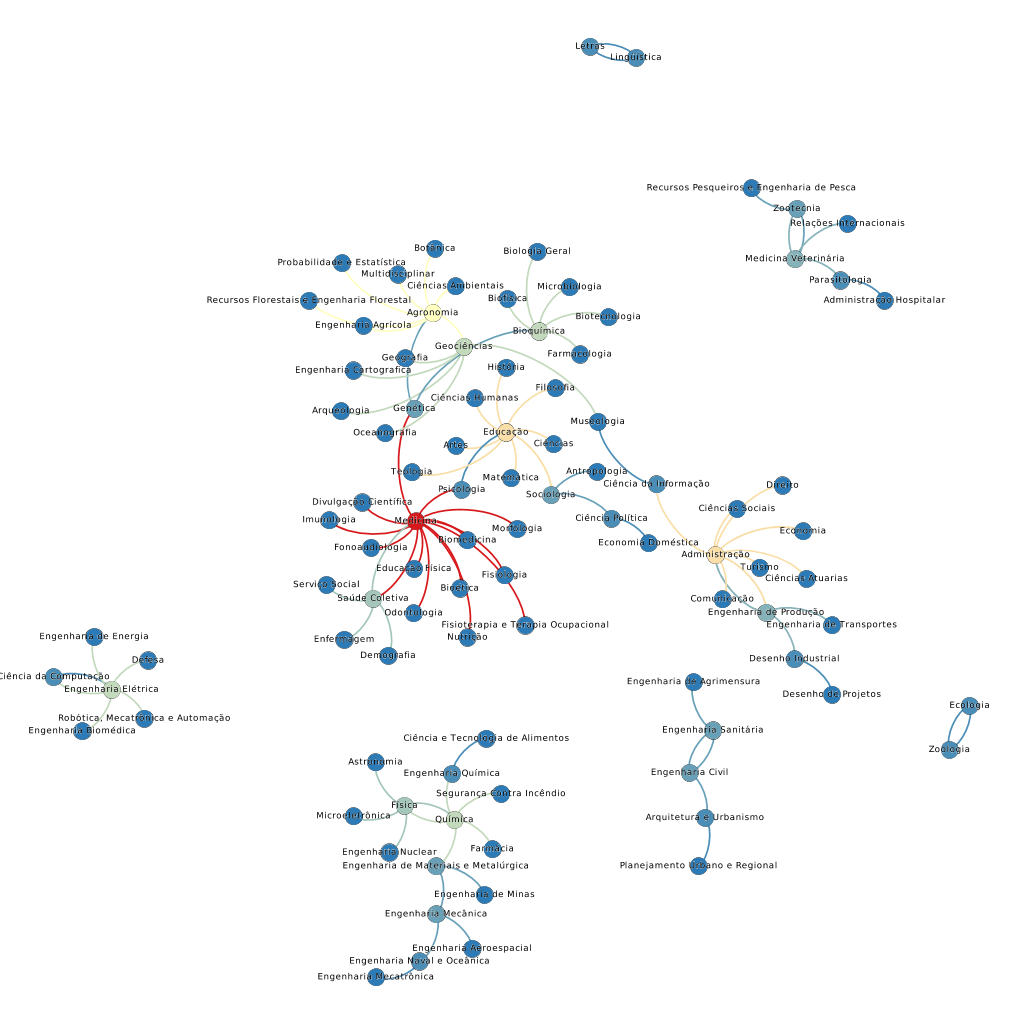
\includegraphics[width=1\textwidth]{figuras/resultados-grafo-impacto}
  \caption{Grafo do impacto exercido pela área do conhecimento na produção científica feita em colaboração das outras áreas. Os nós com cores mais quentes são os que mais exercem impacto em outras áreas.}
  \label{fig:grafoimpacto}
\end{figure}

Nele é possível observar que existem $7$ componentes conexas, onde a maior componente conexa conta com 61 nós, o que representa $62,89$\% da rede. A Ciência da Computação faz parte de um subgrafo que está interconectado pela Engenharia da Elétrica. Nele é observado que o impacto exercido pela Ciência da Computação é relevante apenas para a Engenharia Elétrica.

\section{Interdisciplinaridade}

Interdisciplinaridade é um conceito que pode ser interpretado de diferentes maneiras \cite{rousseau2019knowledge}. Neste trabalho uma publicação em coautoria será considerada interdisciplinar se os coautores pertencem a pelo menos 3 áreas distintas.

O número de publicações científicas interdisciplinares feitas em coautoria apresentado na \autoref{tab:producaointerdisciplinar} mostra que a Ciência da Computação, apesar de construir muitas publicações em coautoria, não tem muita atuação em projetos interdisciplinares.

\begin{table}[htpb]
    \centering
    \caption{As 20 áreas com o maior número de publicações interdiscplinares.}
    \label{tab:producaointerdisciplinar}
    \begin{tabular}{|r|l|c|}%
        \hline & Área & Número de publicações interdisciplinares\\\hline
        \csvreader[late after line=\\\hline]%
        {"tabelas/resultados-producao-bibliografica-interdisciplinar.csv"}%
        {area=\area,contagem=\contagem}%
        {\thecsvrow & \area & \contagem}%
    \end{tabular}
\end{table}

A Medicina aparece como a área com mais publicações feitas em grupos interdisciplinares, são $37.578$ das suas $565.761$ publicações feitas em coautoria. Todavia, este número ainda representa pouco mais de $6,5$\% das suas publicações.

Podemos ver na \autoref{tab:producaogrupointerdisciplinar} que a maioria das publicações da Ciência da Computação feitas em coautoria são realizadas apenas com pesquisadores de mais uma área do conhecimento. O mesmo comportamento também é observado na Medicina, Agronomia, Educação e Química, o que sugere que as publicações interdisciplinares não são muito comuns. 

\begin{table}[htpb]
    \centering
    \caption{Número de publicações onde os grupos com pesquisadores Ciência da Computação eram compostos por pesquisadores de outras áreas.}
    \label{tab:producaogrupointerdisciplinar}
    \begin{tabular}{|r|r|}%
        \hline Número áreas diferentes & Contagem de publicações \\\hline
        \csvreader[late after line=\\\hline]%
        {"tabelas/resultados-producao-bibliografica-computacao-e-grupos-interdisciplinares.csv"}%
        {tamanhodogrupo=\tamanhodogrupo,contagem=\contagem}%
        {\tamanhodogrupo & \contagem}%
    \end{tabular}
\end{table}
